% !TEX program = xelatex
% !TEX options = --shell-escape -synctex=1 -interaction=nonstopmode -file-line-error "%DOC%"
% \documentclass[handout]{beamer}
\documentclass{beamer}

\usetheme{Madrid}
\usecolortheme{default}

\usepackage{ctex}
\usepackage{listings}
\usepackage{multicol}
\usepackage{verbatim}
\usepackage{amsmath}
\usepackage{amsfonts}
\usepackage{amssymb}
\usepackage{mathrsfs}
\usepackage{bm}
\usepackage{pdfpages}

\newcommand{\ud}{\mathrm{d}}
\newcommand{\mev}{\mathrm{MeV}}
\newcommand{\gev}{\mathrm{GeV}}

\title[Identify]{$\alpha \beta$ Particle Identification}
\author[xOasis]{徐大成 \and 武益阳}
\institute[THU]{清华大学}
\date{2020.05.31}

\AtBeginSection[]
{
    \begin{frame}
        \frametitle{Overview}
        \tableofcontents[currentsection]
    \end{frame}
}

\begin{document}
\frame{\titlepage}

\begin{frame}
\frametitle{Overview}
\tableofcontents
\end{frame}

\section{算法}

\begin{frame}
\frametitle{CNN}
\begin{itemize}
    \item 首先尝试了球面卷积神经网络(Spherical CNN, S2CNN)
\end{itemize}
\end{frame}

\begin{frame}
\frametitle{球面卷积神经网络试验}
如果我们希望从切伦科夫环的角度来进行粒子判别,针对探测器的球面流形进行神经网络显得更加自然、有物理意义。我们尝试了使用S2CNN,主要有以下几步:
\begin{enumerate}
    \item <1-> 将PMT的位置转化为方位角坐标$(\theta, \varphi)$
    \item <2-> 在$(\theta, \varphi)$相空间构造一个30$\times$30的格点,30个PMT位置就在30个格点上,值为该事例在该PMT上响应出的电荷。
    \item <3-> 使用30个PMT的位置作为卷积核(一个球面流形卷积核),遍历离散化的SO(3)群元素:将每个SO(3)作用到卷积核上,卷积核被旋转;旋转后的卷积核与输入层做内积,作为一个输出。遍历完成后输出一个在SO(3)空间的张量。
    \item <4-> 如法炮制,只不过这次卷积核是SO(3)的一些格点。
    \item <5-> 卷积结果最终线性映射回到粒子判别上
\end{enumerate}
\end{frame}

\begin{frame}
\frametitle{球面卷积神经网络试验}
\begin{figure}[H]
    \centering
    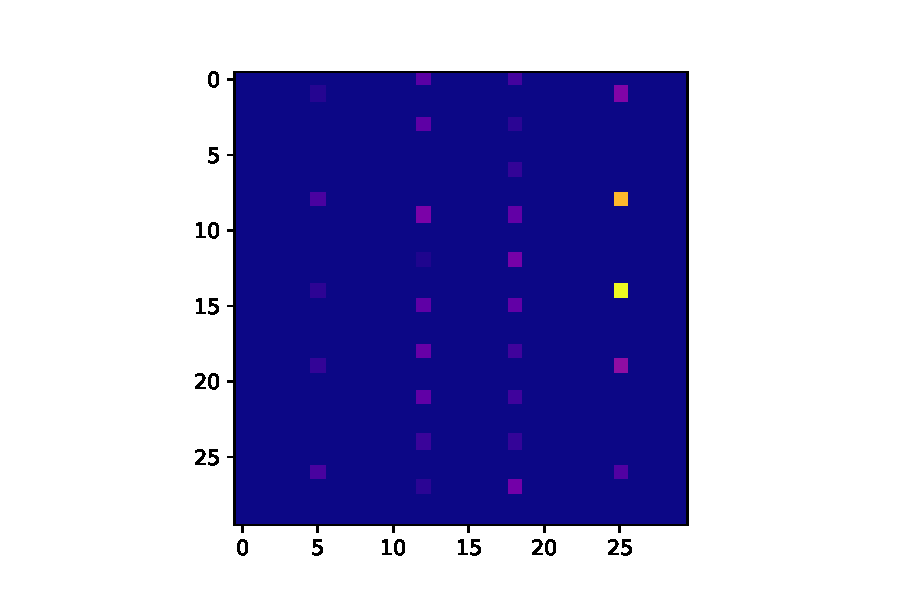
\includegraphics[width=0.6\textwidth]{S2CNN_input.pdf}
    \caption{S2CNN输入层:PMT电荷}
    \label{fig:S2CNN_input}
\end{figure}
该方法没有效果,训练结果与随机猜测无异。
\end{frame}

\begin{frame}
\frametitle{平面二维卷积神经网络}
\begin{itemize}
    \item <1-> 随后设计了一个7层卷积神经网络(CNN)
    \item <2-> Inputs:30个PMT在1029ns的采样时间内的ADC电压输出($1029\times30$)
    \item <3-> Outputs:对$\alpha$与$\beta$两种粒子的预测概率
    \item <4-> 使用stride迅速缩小Outputs的大小
    \item <5-> 网络中总参数为81526个
    \item <6-> Activation Function:LeakyReLU($\alpha=0.1$)
    \item <7-> 输出层:Softmax
    \item <7-> Loss:交叉熵函数(Cross entropy)
\end{itemize}
\end{frame}

\begin{frame}
\frametitle{平面二维卷积神经网络}
\begin{figure}[H]
    \centering
    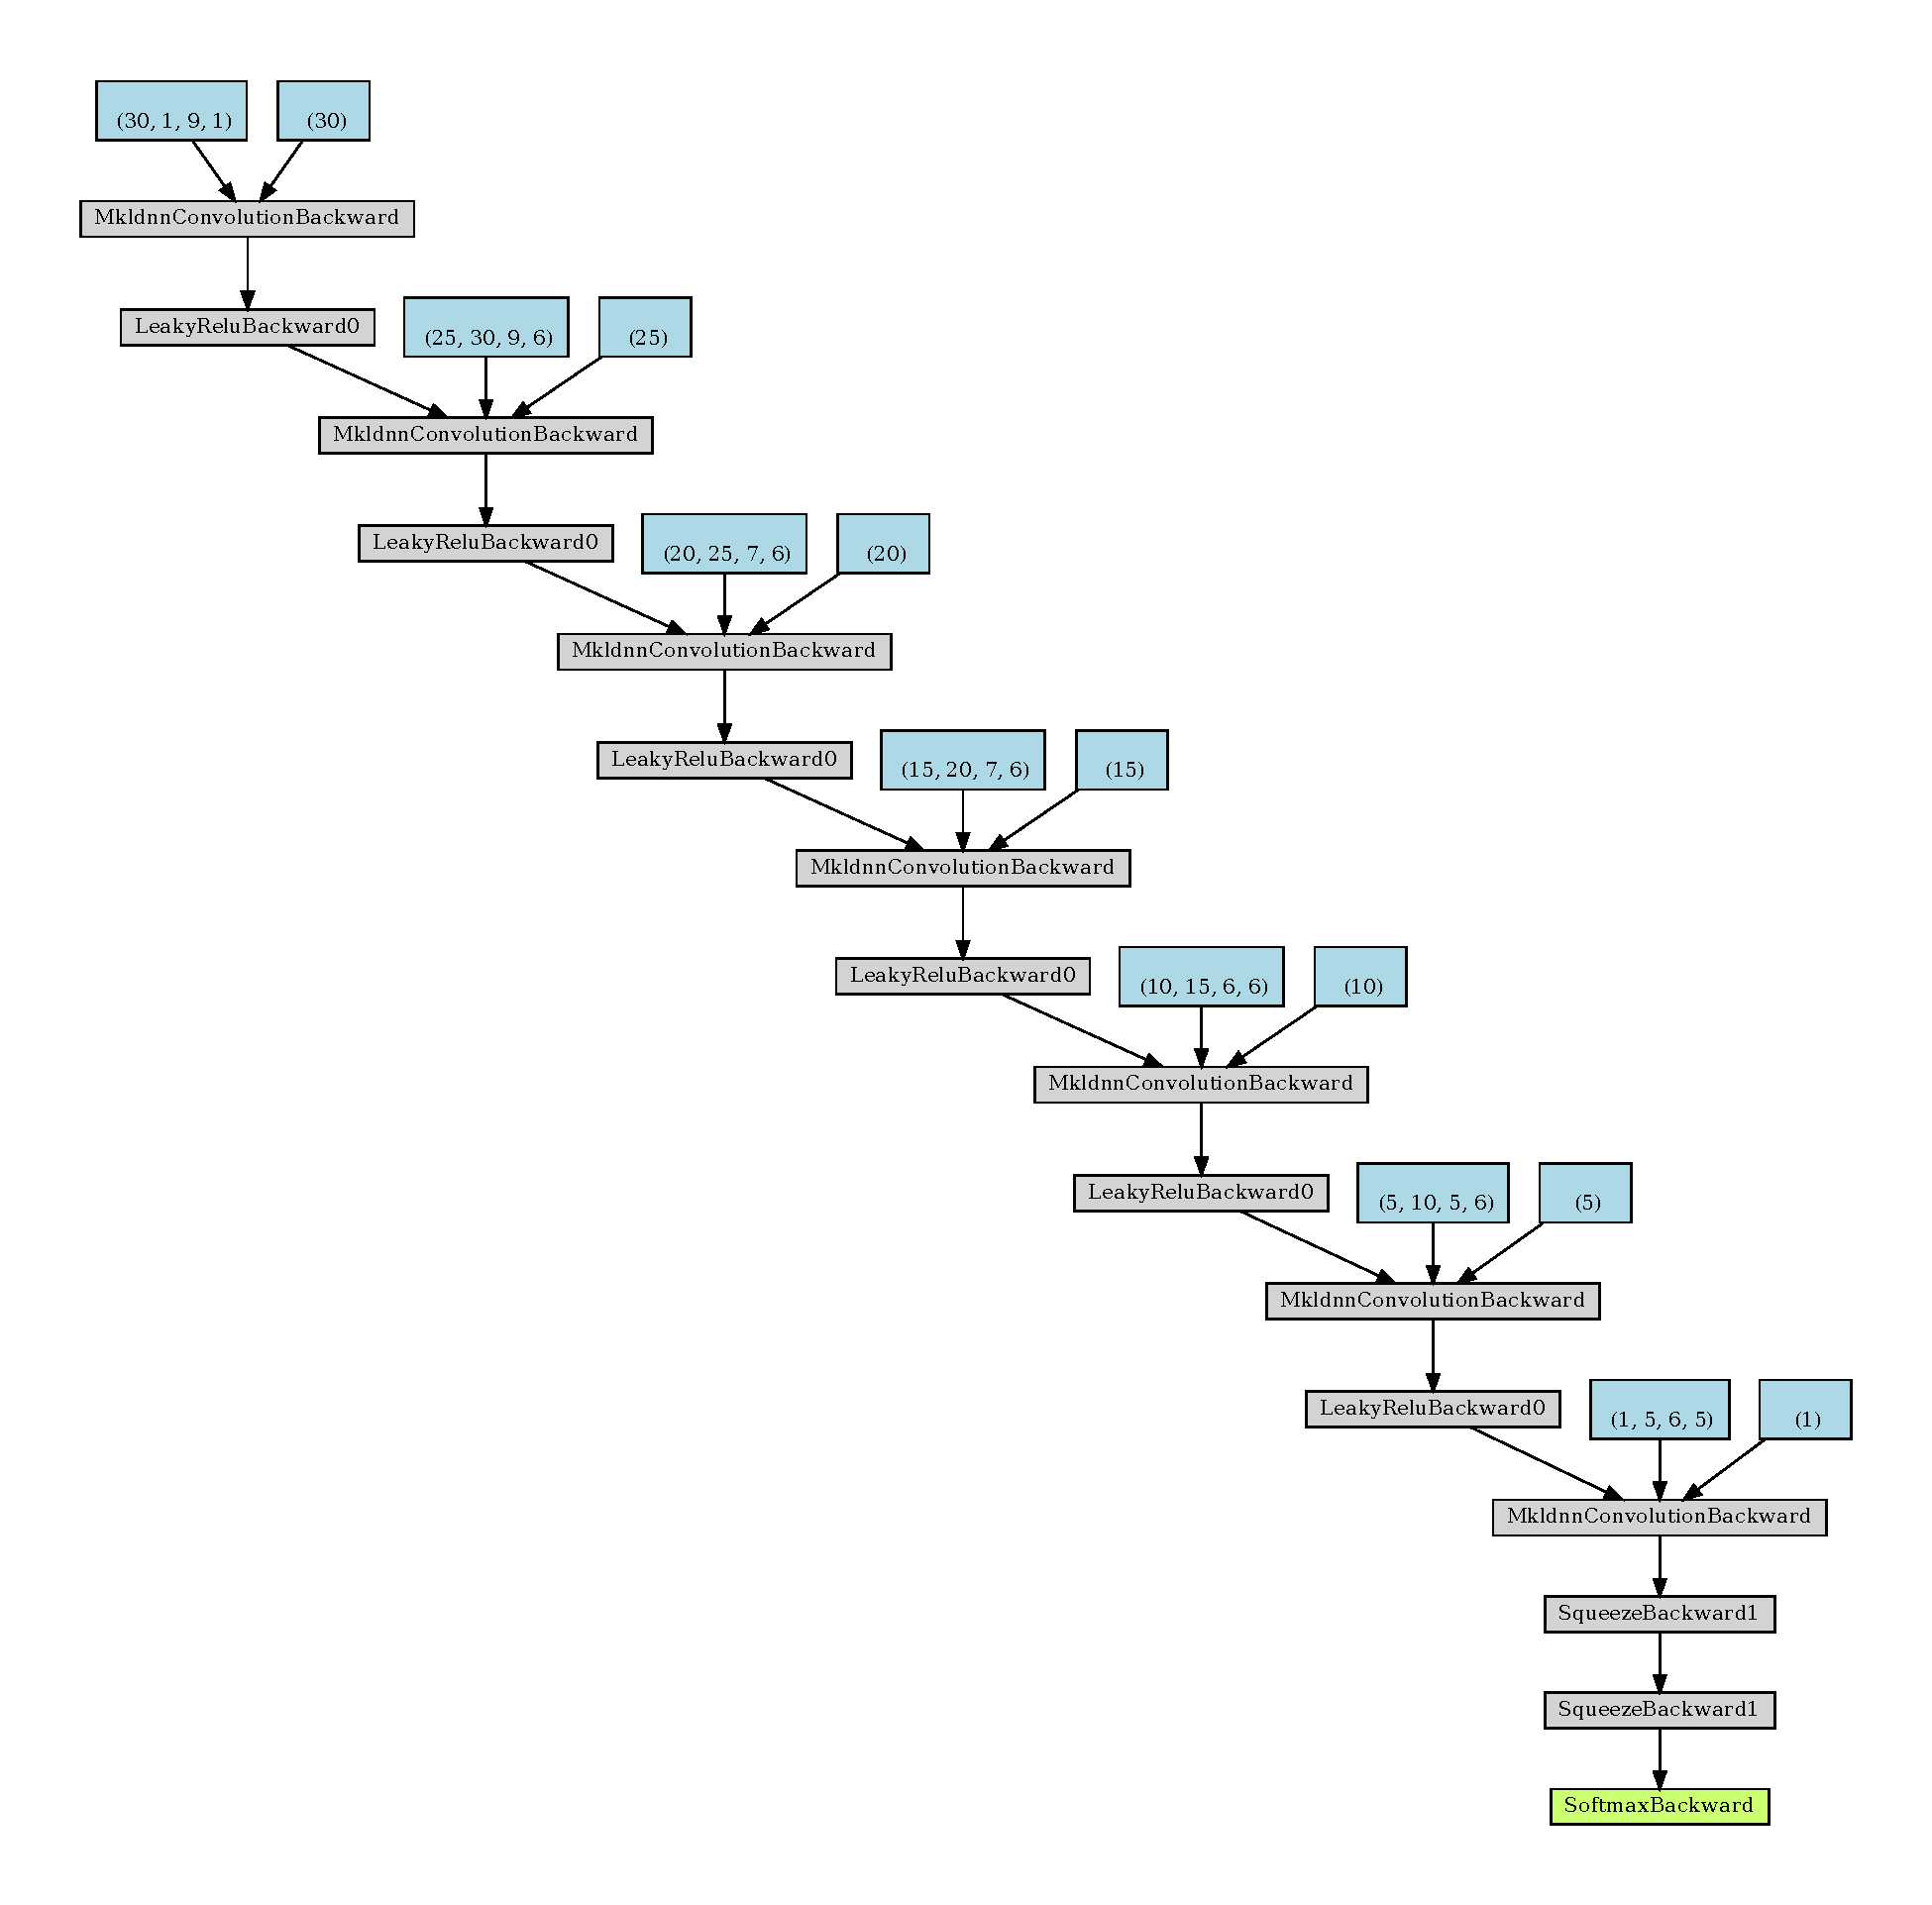
\includegraphics[width=0.6\linewidth]{net.pdf}
    \caption{CNN结构}
\end{figure}
\end{frame}

\section{算法检测结果}
\begin{frame}
\frametitle{算法检测结果}
\begin{columns}
\column{0.5\textwidth}
\begin{figure}[H]
    \centering
    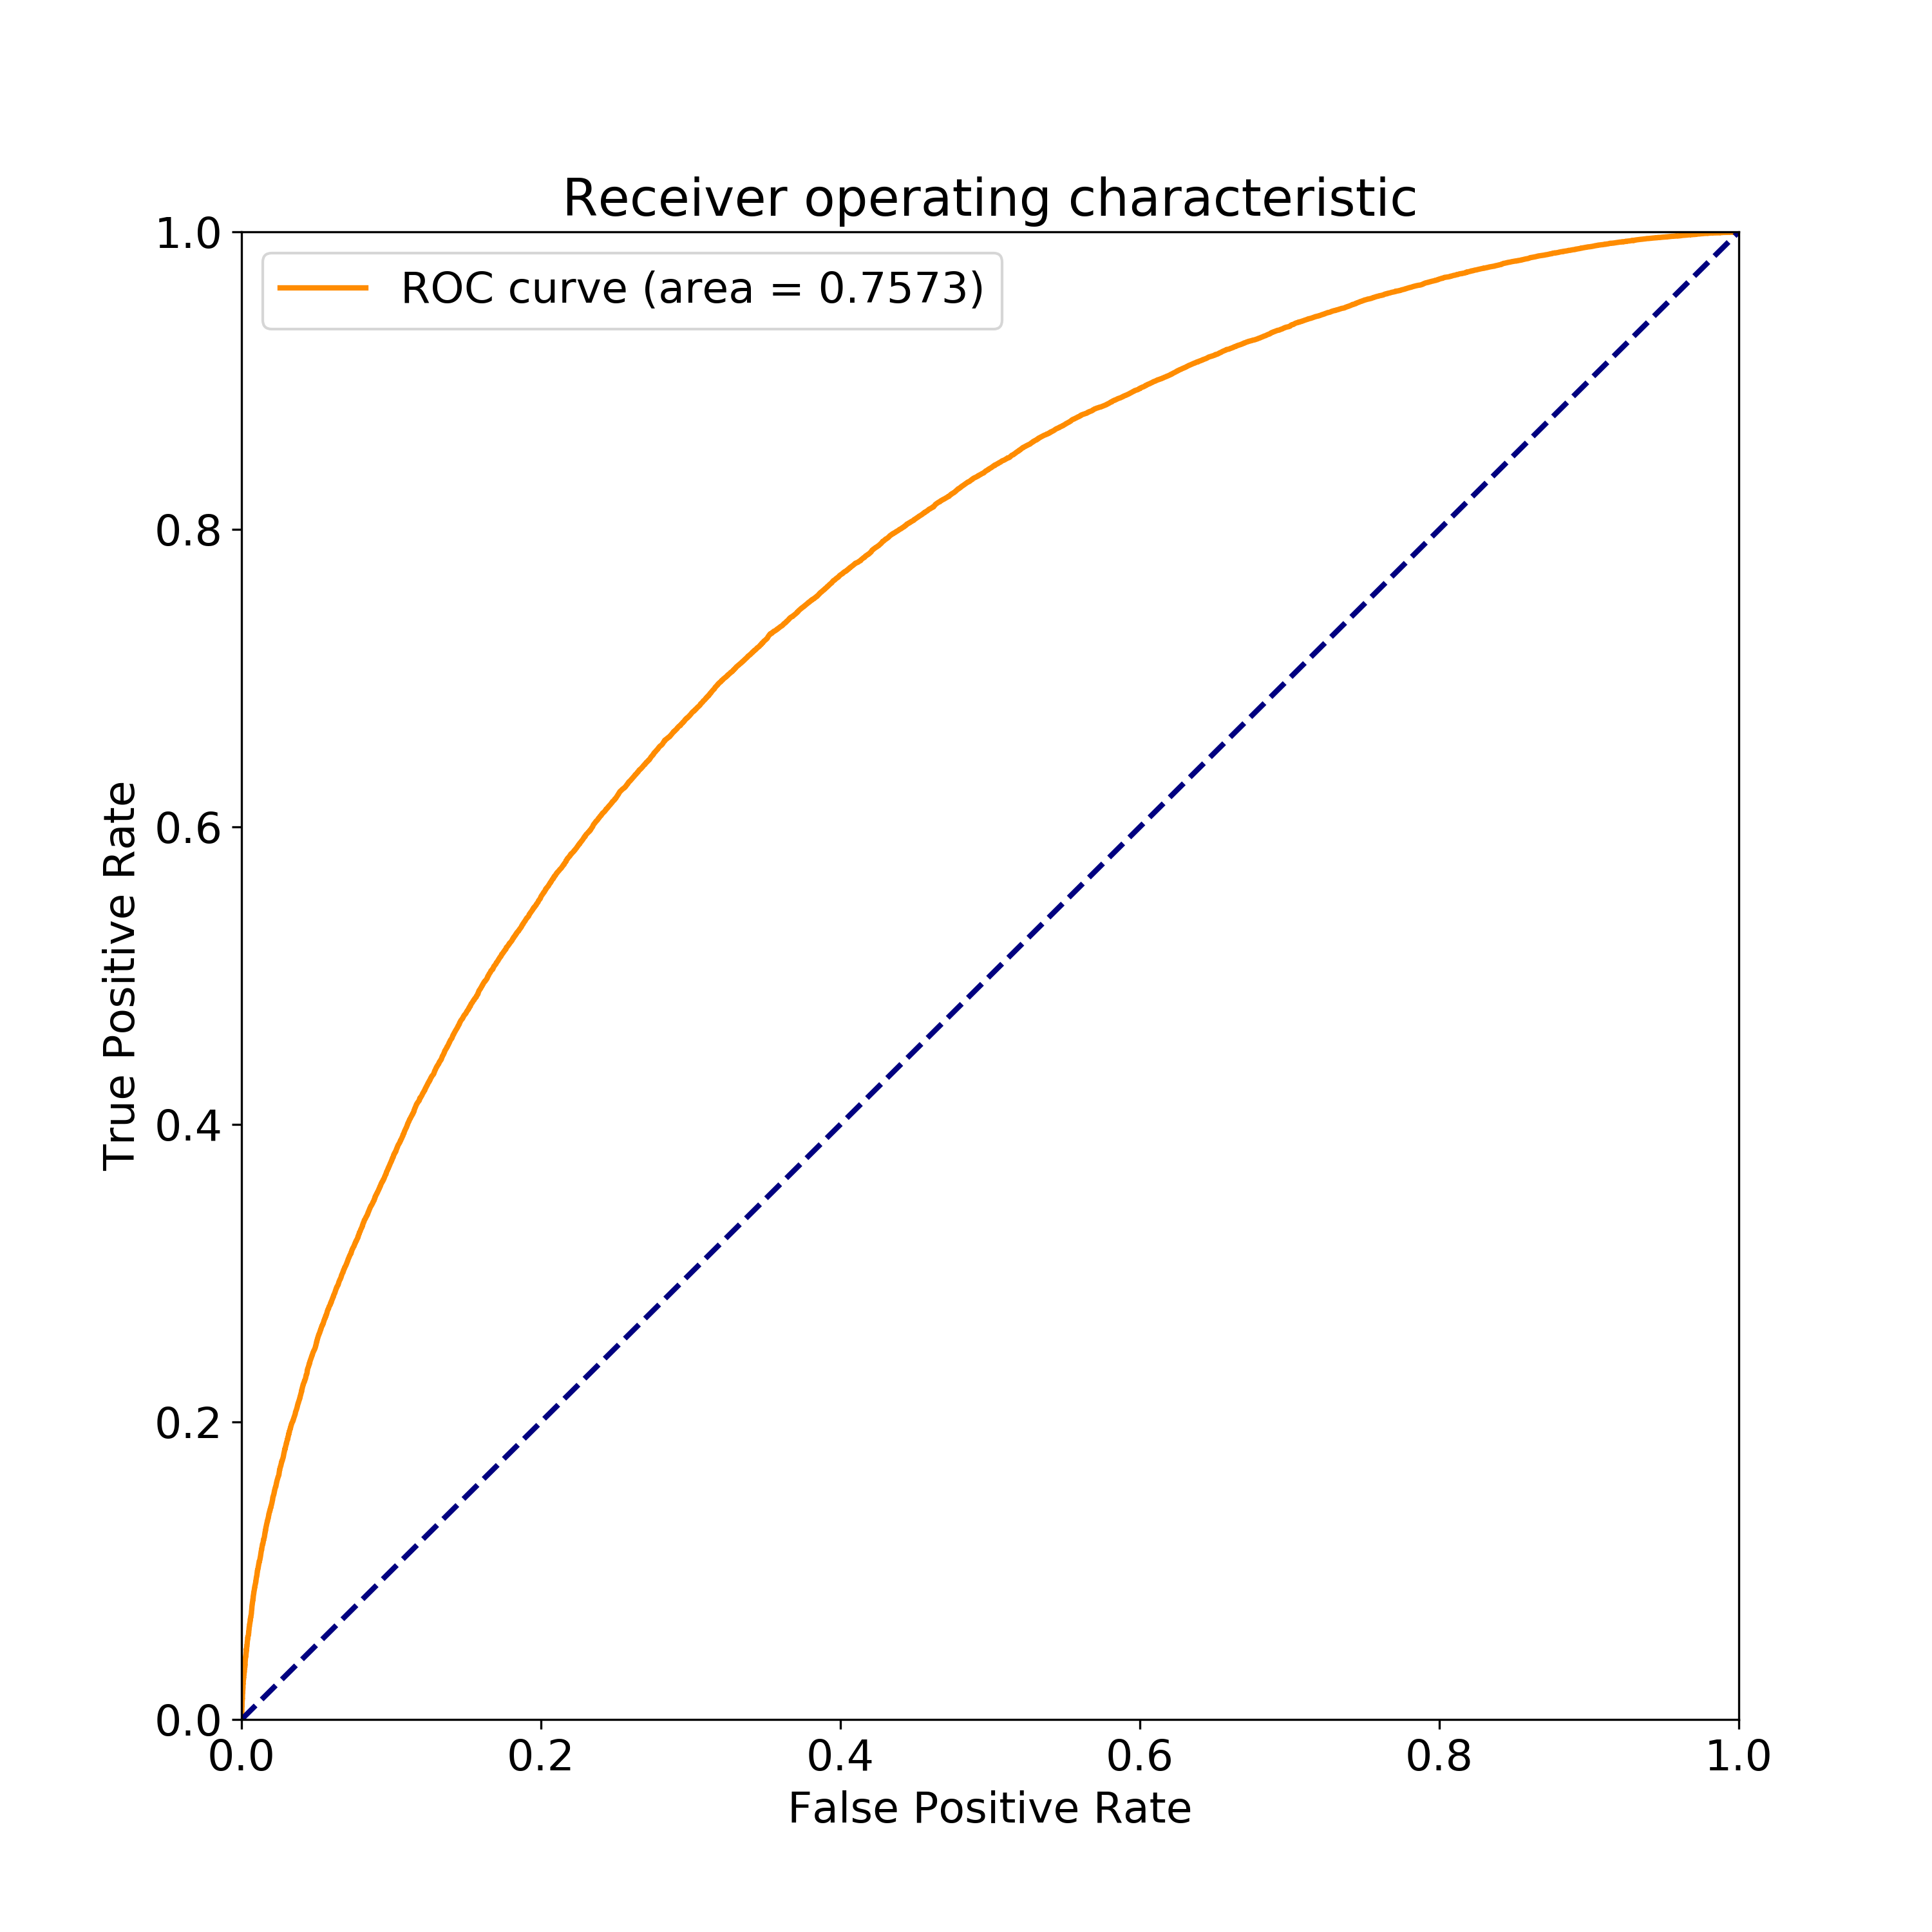
\includegraphics[width=1.0\linewidth]{ROC.png}
    \caption{CNN在final-0.h5上的ROC曲线}
\end{figure}
\column{0.5\textwidth}
\begin{itemize}
    \item 测例:final-0.h5显卡进行处理
    \item 环境:NVIDIA GeForce GTX 1080Ti
    \item 用时:3.4min(包括CPU时间)
    \item AUC:0.7573
\end{itemize}
决赛中:
\begin{itemize}
    \item 在Ghost Hunter2020决赛中对final-problem.h5处理
    \item 环境:NVIDIA GeForce GTX 1080Ti
    \item 用时:4min(包括CPU时间,不包括预处理)
    \item 预处理:1.5min
    \item AUC:0.748,(6th)
\end{itemize}
\end{columns}
\end{frame}

\section{改进}
\begin{frame}
\frametitle{改进}
\begin{itemize}
    \item 在制作训练集的过程中没有对PMT输出电压进行任何处理。在减去基线后,可能对CNN训练及预测结果有一定提升
    \item 激活函数LeakyReLU的参数选取中,只测试了$0.05$和$0.1$。可以通过交叉验证来优化激活函数
    \item $\cdots$
\end{itemize}
\end{frame}

\end{document}